
\chapter[]{Modularisation des systèmes distribués}% TODO: maybe rename.
%%% - Programme/Processus
%%% - Exécutable

Les programmes modernes ont une structure \textit{modulaire},
c'est-à-dire que leur code se décompose logiquement en différentes
parties relativement indépendantes, les \textit{modules}.  Cette
structure a de nombreux avantages, entre autres sur le plan du
développement et de la maintenance.  La structure d'un programme en
vue de son \textit{déploiement} -- c'est-à-dire comment son code
exécutable est stocké sur disque, chargé en mémoire, etc. -- peut prendre
plusieurs formes.

Un programme sous forme \textit{monolithique} contient dans son code exécutable
toutes les instructions exécutées par l'ordinateur.  Cette forme était la norme
dans les premiers systèmes informatiques, et l'est toujours pour les systèmes
embarqués qui n'ont pas de système d'exploitation indépendant.  Lorsqu'un
système d'exploitation est disponible sur l'ordinateur on peut le considérer
comme étant un module puisqu'il offre des services précis avec une interface
standardisée.  Dans ce cas, un programme peut prendre la forme d'un seul
fichier de code qui, à son exécution, communiquera avec le système
d'exploitation pour accéder à ses services.  Ce genre de fichier exécutable est
obtenu par une \textit{édition de liens statique} qui combine en un seul
fichier tous les modules (à l'exception du système d'exploitation).  Par
rapport à la forme monolithique, cette organisation simplifie le développement
car le programmeur n'a pas à se soucier du développement des services de base
comme l'accès aux fichiers, la gestion des processus et de la mémoire, etc.  Le
programme peut être distribué à d'autres ordinateurs ayant le même système
d'exploitation simplement en y transférant le fichier exécutable.

L'édition de lien statique a un certain nombre de défauts. La version des
modules utilisé au moment de l'édition de liens est figée au sein du
programme, ce qui empêche la mise à jour individuelle des modules. Il faut
recompiler tous les modules qui ont subi une mise à jour et refaire l'édition de liens du
programme principal. Le coût en temps et l'effort pour un changement minime
est important.  Le chapitre \ref{ch:loading-model} va détailler plus en profondeur
ces problèmes.

% Le même module est chargé plus d'une fois.
L'édition de liens peut se faire paresseusement par le système d'exploitation à
l'exécution du programme, ce qu'on appelle l'\textit{édition de liens dynamique}.  Cela
permet de garder la structure modulaire au \textit{déploiement}.
Chaque module est une composante séparée du programme principal.  Ces modules
sont lu du disque et chargés en mémoire durant l'exécution du programme.  Ce
chargement est effectué par \textit{éditeur de liens dynamique} qui s'occupe de
lié les fonctionnalités des modules au programme principal. Le chapitre % chapter or section
\ref{ch:loading-model} explique plus en profondeur le fonctionnement de éditeur de liens
dynamique. L'avantage principal du chargement dynamique de module est la mise à jour
individuelle d'un module sans avoir a lié le programme principale; dans le
modèle statique le programme principal doit être lié à nouveau avec les modules.
Les modules chargés dynamiquement par le système d'exploitation peuvent être partagé entre différent
programme. Ce type de module porte le nom de \textit{bibliothèque partagée} ils sont décrit dans
le chapitre \ref{ch:loading-model}.

% % Migration de code dans un système distribué.
% - Transmission de tâche entre des machines d'un système distribué.
%   - Un module absent sur la machine distante nécessaire à l'exécution
%   de la tâche transmise.
%     - Télécharger le module d'un serveur dédié.
%     - Revient au chargement dynamique de ce module.

Dans un système distribué, il est possible de transmettre des tâches entre les
différents systèmes. C'est ce qu'on appelle, \textit{migration de tâche}.  Un
programme distribué est séparé sur plusieurs systèmes. Qu'est-ce qui se passe
si une tâche transmit réfère à un module absent sur le système distant?  Le
système distant peut soit lancé une exception, ou tenté de résoudre la
fonctionnalité manquante. La première solution est la plus simple et aussi la
plus restrictive, car elle inhibe la capacité de migrer une tâche. Le chapitre
\ref{ch:task_migration} traite de la seconde solution mentionné.

% \section{Linkage statique}
% Cette forme d'édition de lien permet la création de binaire qui indépendant
% qui facilite le déploiement.

%\section{Linkage dynamique}

--------------------------END---------------------------

% TODO: move to chapter task_migration
Un programme sur une des machine du système distribué qui se fait transmettre
une tâche peut devoir exécuter une fonctionnalité d'un module absent
localement. Cela nécessite un téléchargement du module contenant la
fonctionnalité demandé d'un serveur dédié. Une fois le module installé, il faut
le charger dynamiquement.

==> motiver (quels problèmes ça cause le link statique) et expliquer le chargement dynamique, système distribué, etc
% TODO lien => liens


%Problème du link statique\\
% - Gèle les versions des modules au sein du programme. \\
%    -> Comment la maintenance d'un programme lié statiquement? \\
%    - Le temps de compilation. (Coût d'un changement est important) \\
% - La taille du programme peut être plus importante.
% - Le même module est chargé plusieurs fois en mémoire.

--------------------------------------------------------


Dans les systèmes comme DOS, les programmes ou modules devaient contenir toutes les
informations nécessaire pour s'exécuter. De tels programmes sont dit lié
statiquement dans le sens qu'il ne dépende que de l'architecture sur laquelle il
a été construit. La construction des modules requière deux étapes. La compilation
de fichier source en fichier objet contenant le nom et le code des fonction.
L'édition des liens qui réunit un plusieurs fichiers objets en un module.
Dans le cas d'un seul fichier l'édition des liens ne fait que transformer le fichier
objet en fichier exécutable.

\begin{figure}[ht]
  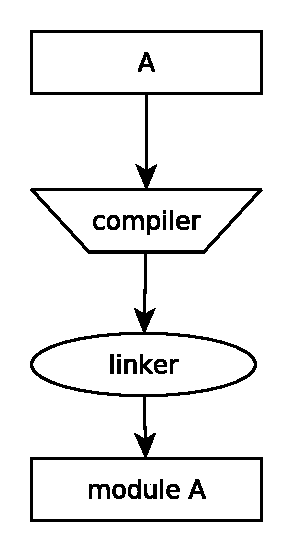
\includegraphics[width=0.20\linewidth]{figures/basic_module_compilation.pdf}
  \caption{Construction du module A à partir des sources.}
\end{figure}

%La création d'exécutable inclut deux étapes importantes, la compilation et
%l'édition des liens. La première étape consiste à prendre un fichier de code
%source et de le traduire en fichier objet, que l'on retrouve souvent avec
%l'extension \verb|.o| ou \verb|.obj|, qui contient la représentation des
%procédures compréhensible par le processeur. Ces fichiers objets ne sont pas
%encore exécutable pour autant, il faut tout d'abord effectuer la seconde étape,
%qui va les regrouper en un exécutable. Le programme qui s'occupe de l'édition
%des liens est le \textit{linker}, la version GNU se nomme \verb|ld|.  Voici
%l'exemple de la création d'un exécutable composé des fichiers sources C
%\verb|main.c| et \verb|foo.c|:
%
%\begin{figure}[ht]
%    \begin{minipage}[t]{0.5\textwidth}
%\begin{verbatim}
%# Compilation
%gcc -c main.c -o main.o
%gcc -c foo.c -o foo.o
%# Édition de liens
%ld -o main.exe main.o foo.o
%\end{verbatim}
%    \end{minipage}
%
%    \caption{Exemple de création d'un exécutable}
%\end{figure}

Pour permettre la réutilisation de code et faciliter
l'écriture de programme plus complexe, le concept de bibliothèque de code est
apparu. Par la contrainte des systèmes, le premier type de bibliothèques utilisé
étaient dit statique.  Elles consistaient en un regroupement logique de
plusieurs fichiers objets en un archive (.a). La création d'une bibliothèque
statique peut s'effectuer avec l'utilitaire \verb|ar|. Lorsque que programme se
lie à une bibliothèque statique, il inclut tout simplement l'ensemble des
procédures contenu dans les fichiers objets. L'avantage des bibliothèques
statiques est de regrouper plusieurs fonctionnalité commune en un seul concept,
par exemple la bibliothèque mathématique \verb|libm.a| qui contient les
fonctions mathématique (i.e. \verb|cos|, \verb|sin|).  En plus,  fait que le
processus d'édition des liens, qui consiste à associer les noms des
fonctionnalités avec leur valeur (AMBIGU), n'est effectué juste une fois. Une
liaison avec une bibliothèque statique \verb|libfoo.a| qui contient le fichier
objet \verb|foo.o| est équivalent à une liaison directe avec le fichier
\verb|foo.o|.

\begin{figure}[ht]
    \begin{minipage}[t]{0.5\textwidth}
\begin{verbatim}
# Création de la bibliothèque statique libfoo.a
ar rcs libfoo.a foo.o
# Création de l'exécutable main.exe
ld -o main.exe main.o libfoo.a
\end{verbatim}
    \end{minipage}

    \caption{Exemple de création de bibliothèque statique suivit d'un exemple
    d'utilisation.}
\end{figure}

\todo{Citation}
Un des problèmes des bibliothèques statiques le coût est lié à la maintenance.  Les
programmes qui utilise des bibliothèques statiques ne permettent pas une
construction modulaire. La mise à niveau d'une des bibliothèques statiques
nécessite la recompilation du programme au complet. En plus, cela n'est pas
adapté pour des application d'un application évolutif qui peuvent être étendu
par l'utilisateur. Une solution qui a été adopté est le
concept des bibliothèques partagés (ou dynamique). Cela offre une plus grande
liberté dans la conception des programmes. Un programme qui ce lié avec une
bibliothèque partagé ne contient pas les définitions importé de la
bibliothèque, seulement l'information pour la trouvé. Cette information
consiste généralement aux noms de la fonctionnalités utilisé et des
bibliothèques dépendantes. Contrairement aux bibliothèques statiques,
l'édition des liens s'effectue à chaque exécution du programme.
Les bibliothèques partagés offre plusieurs avantages par rapport
aux bibliothèques statique.

La construction d'un programme peut s'effectuer de façon modulaire; chaque
composantes du programme peuvent être construites en séparément.  La
modification d'une des bibliothèques partagés utilisés par
le programme ne nécessite pas la recompilation de celui-ci. Le nom qui est
donné à l'entité qui résout les noms des fonctionnalités est l'éditeur de liens (\textit{dynamic linker}).
Habituellement les bibliothèques exportent des fonctions, mais il peuvent aussi
exporter plusieurs types de données comme des entiers, des nombres à virgules,
des chaînes de caractères et des données composites (structures). Chacune de ces données est
associées à un nom unique (symbole) au sein de la bibliothèque.
Il n'est pas possible d'avoir deux bibliothèques statiques qui exportent une
fonctionnalité avec le même nom au sein d'une même application, alors qu'avec
les bibliothèques partagés c'est possible. Cela limite le choix des
bibliothèques qui peuvent être utilisé simultanément au sein du programme;
chaque bibliothèque doit avoir un ensemble de nom de fonctionnalité distinct
des autres. Puisque la résolution d'une fonctionnalité retourne la première
occurrence trouvée, il n'y a rien qui empêche d'avoir plus d'une fonctionnalité
associée au même nom.

Gambit permet de l'utilisation de bibliothèques statiques et dynamiques.
Chaque fichier Scheme peuvent être compilé et lié module exécutable ou
en bibliothèque dynamique.

\begin{center}
\begin{figure}[ht]
  \begin{tabular}{l}
    \begin{mplisting}{0.5}
;; fib.scm
(define (fib n)
  (if (< n 2)
      n
      (+ (fib (- n 1))
         (fib (- n 2)))))
\end{mplisting}
  \end{tabular}
  \caption{Un module qui implémente la fonction mathématique \texttt{fib}.}
  \label{fig:basic_fib_module}
\end{figure}
\end{center}

\vspace{-20pt}
La construction d'un bibliothèque dynamique à partir du fichier \texttt{fib.scm}
de la figure \ref{fig:basic_fib_module} s'effectue par le compilateur de Gambit
qui nomme \texttt{gsc}. Cela produit un fichier avec l'extension \texttt{.oN}
où le \texttt{N} correspond à la version généré de la bibliothèque qui commence à 1.

% NOTE: distingué version .oN et version du code.

\section{Coexistence entre bibliothèque}
Les bibliothèques coexistent de deux façon principales, de façon passive dans
un système fichier et de façon active durant l'exécution d'un programme.  Un
système de fichier contient un arborescence hiérarchique de répertoires et de
fichiers avec une seule racine. Un fichier est l'entité dans un système de
fichier qui contient les données, c'est dans cette entité que le code des
bibliothèques ce situe.  Les répertoires sont les entités qui permette de
regrouper plusieurs fichiers de façon logique. La racine correspond au sommet
de la hiérarchie du système de fichier. La façon de référer au un fichier
uniquement dans un système de fichier est d'utiliser le chemin absolu. Cela
correspond à la liste des répertoires à parcourir de la racine jusqu'au
fichier. L'outil responsable d'organiser les bibliothèques sur un système
est le \textit{package manager}. Il possède plusieurs objectif incluant
l'installation de bibliothèque, la mise à jour de toute les bibliothèques
installées, la désinstallation de bibliothèque et la résolution des dépendances.

Un cas intéressant de coexistence entre bibliothèques est celui qui inclue
plusieurs versions d'une même bibliothèque, car cela peut amener des problème
à la fois sur le système de fichier et durant l'exécution d'un processus utilisant
ces bibliothèques. Il y a aussi plusieurs utilités d'avoir plusieurs version
d'une même bibliothèque, cela permet de supporter des application qui dépend de
bibliothèques antérieurs.

Un autre application est de convertir un vieux format de fichier vers un format
plus récent. Dans le cas où il n'est pas possible de plusieurs version d'une bibliothèque
il faut alors écrire un \textit{reader} pour lire le vieux format manuellement ensuite le
utilise fonctions de la version cible de bibliothèque pour générer le nouveau format du fichier.
Cette solution à comme problème que le \textit{reader} est beaucoup moins testé que la
vielle version de la bibliothèque. Cela demande aussi de réécrire qu'est-ce qui à déjà été fait.

\begin{figure}[ht]
  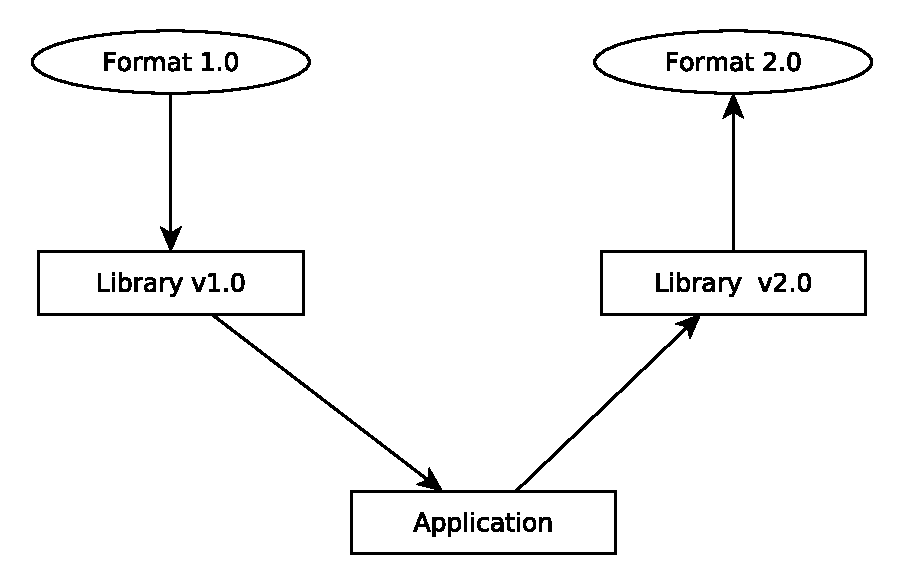
\includegraphics[width=30em]{figures/app_convert_v1_to_v2.pdf}
  \caption{Un exemple d'application de conversion entre deux version d'un format
  de fichier comme sqlite2 et sqlite3 exploitant la possibilité de charger plusieurs
  version d'une bibliothèque.}
\end{figure}

L'architecture de processus sur un système permet plusieurs propriétés. La
robustesse, un processus failli les autres processus ne sont pas affectés. La
sécurité et l'isolation, chaque processus possède leur mémoire qui n'est pas
accessible par les autre processus et peuvent utilisé une version spécifique
des bibliothèques. Il est possible de concevoir l'architecture de processus en
utilisant des threads.  Un \textit{thread} décrit un courant d'exécution d'un
programme. Un processus à au minimum un \textit{thread} qui correspond au
courant d'exécution principal du programme. Les \textit{threads} sont utiles
pour paralléliser l'exécution d'un processus. La création de \textit{threads}
est beaucoup plus rapide que la création d'un processus, car elle ne nécessite
pas l'appel au système d'exploitation.

Ce modèle exploite la légèreté des \textit{threads} par rapport au processus et
la possibilité de charger plusieurs version des bibliothèques qu'il a besoin au sein
du système. Cela est similaire au modèle de processus utilisé par les
système d'exploitation, sauf que l'ensemble est juste au sein d'un seul processus.
Étant donnée que les \textit{threads} vivent tous au sein d'un même processus,
il est donc facile de partagé des informations d'un \textit{thread} à un autre.
Ce qui est plus difficile avec le modèle de processus, cela nécessite l'utilisation
mécanisme comme la mémoire partagé.

%\todo{picture: Thread as Light process}

% TODO: exemple de chemin.

%et s'il c'est un cas qui peut
%contenir un coexistence néfaste.  Cela n'est possible que s'il est possible de
%distinguer les deux version de la bibliothèque et aussi répartir les appels à
%des fonctions de même nom à la bonne version de la bibliothèque.


\subsection{Coexistence au sein d'un processus}
L'autre type de coexistence entre les bibliothèques est durant l'exécution d'un
processus.  La coexistence entre des bibliothèques peuvent être positive ou
néfaste.  Un coexistence positive entre des bibliothèques est marqué par une
bonne répartition des appels de fonctions parmi ces bibliothèque.  Un appel à
la fonction \verb|foo| de la bibliothèque \verb|libA.so| ne va pas être
effectué dans la bibliothèque \verb|libB.so|. Deux bibliothèques ne coexiste
pas correctement au sein d'un processus si les appels de fonctions sont
réparties incorrectement parmi les bibliothèques. Le chargement des bibliothèques
diffère d'un langage interprété à un langage compilé nativement.

\subsubsection{Contexte interprété}
Les bibliothèques dans les langages interprétés utilisent leur propre procédure
de chargement de bibliothèque. Ce processus permet de charger directement les
fonctionnalité d'une bibliothèque à partir du code source.

La façon de charger le code source peut être effectué par une lecture de la
bibliothèque suivit d'un évaluation du code.

\begin{verbatim}
class Module(object):
    def __init__(self, members):
        for k in members.keys():
            setattr(self, k, members[k])

def importFile(name):
    with open(name, 'r') as fd:
        code=fd.read()
    env = {}
    exec(code, env)
    return Module(env)

\end{verbatim}

\subsubsection{Contexte natif}

%\section{Chargement dynamique}
Un des cas probables de deux bibliothèque avec les mêmes noms de fonctionnalité
sont deux versions différente de la même bibliothèque. Il existe des situations
dans lesquelles il serait intéressant d'avoir la possibilité de charger plusieurs
versions d'une bibliothèque.

Il y a dans un système dynamique qui permet de faire une mise à jour du
code sans nécessité un redémarrage du processus. Cet procédure ce nomme
\textit{hot-code-swapping}.

Il y a aussi dans un contexte ou le processus doit supporté plusieurs versions
d'un protocole fournit par une bibliothèque. Par exemple, un application qui migre
le format \textit{sqlite} au format \textit{sqlite3} doit pouvoir charge le fichier
dans le premier format et exporter toutes les tables dans le deuxième format.

\todo{Ajouté plus d'exemple}
